\documentclass[border=5mm]{standalone}
\usepackage{tikz}
\usetikzlibrary{calc}

\begin{document}
\begin{tikzpicture}

\coordinate (m0) at (0,0);
\coordinate (m1) at (-1.0825,-1.875);
\coordinate (m2) at (1.08,0);
\coordinate (m3) at (96.25,0);
\coordinate (m4) at (98.125,-1.875);
\coordinate (m5) at (100,0);
\coordinate (m6) at (100,1.875);
\coordinate (m7) at (66.25,2.5);
\coordinate (m8) at (16.25,2.5);
\coordinate (m9) at (1.0825,1.875);
\coordinate (m10) at (-1.0825,-1.875);
\coordinate (m11) at (100,-3.75);
\coordinate (m12) at (95.25,0);
  \draw (66.25,0) -- (66.25,5);
  \draw (16.25,0) -- (16.25,5);

  \draw (m0) -- (m1) -- (m2) -- (m3)
    -- (m4) -- (m5) -- (m6) -- (m7) -- (m8) -- (m9) --cycle;

\draw[line width=5pt,red] (m9) -- (2, -1.875);
\draw[line width=5pt,red] (m9) -- (m10);
\draw[line width=5pt,red] (m9) -- (m10);
\draw[line width=5pt,red] (m12) -- (m3) -- (m11);
\end{tikzpicture}
\end{document}

